% vim: ft=tex
\chapter{Scope}
The technical goals of this bachelor thesis include extending mindclue GmbH's
Roadster framework by adding features such as clustering, high availability and
transport security. This chapter outlines the general scope of this project.

\section{Motivation}
TODO Why do we care about this thesis? Why are we interested?\\

We're thrilled about the following technologies and software design patterns:

\begin{itemize}
	\item \zmq
	\item Ruby
	\item Actor Model
	\item High Availability
\end{itemize}

Coming from different backgrounds and having different degrees of experience in
each of the above technologies, we can't wait to learn more about them and put
them to actual use. The fact that the product of this bachelor thesis is most
likely going to be used in the real world only adds to the excitement.

In addition to that, we look at this bachelor thesis as an opportunity to
become more fluent in English, as well as a way to improve our skills in
crafting scientific documents using {\LaTeX}.

Depending on how we perform together as a team, further collaboration might
result in the future, either between the students themselves, or between the
students and the client. Even if not, this project will serve as a valuable
reference for future job hunting.

Last but not least, we feel like Prof. Dr. Mehta is a respected and competent
teacher whose opinions we highly value. Due to his polite parlance, discussing
project matters, both of the management and the technical kind, has always been
an enrichment.

\subsection{Open-Source Engagement}
TODO CZTop, cztop-patterns (as mentioned in the Mgmt Summary)

\section{Initial Situation}

\subsection{mindclue GmbH}
\subsubsection{About}
Die Firma mindclue GmbH mit Sitz in Ziegelbrücke GL/SG stellt für ihren
Partner REMTEC AG für Steuerungen, Regelungen und Überwachungen von technischen Prozessen,
komplette SCADA- und Steuerungssysteme her. Dabei sind sie in den Bereichen
Betriebs-und Sicherheitausrüstung für Nationalstrassen, Trinkwasser-
versorgungen, im Energiesektor und vielen Spezielbereichen tätig.
Dabei setzen sie auf ihre eigens entwickelte Applikation - Roadster.

\subsubsection{Roadster}
Roadster ist eine Ereignis gesteuerte Applikation geschrieben in Ruby.
Sie ist die eigentliche SCADA Applikation und wird bereits in einer Vielzahl von
Tunnelanlagen in der Schweiz eingesetzt und dient zur Überwachung der einzelnen Komponenten im Tunnel.
Durch den modularen Aufbau kann jede Roadster Applikation sich selbst laufen - Autonom.
Sprich jeder Roadster hat seinen eigenen Webserver und Datenverwaltung.

\subsubsection{AS - UeLS}
Roadster ist einer von vielen AS Knoten eines UeLS. Die Kommunikation
zwischen AS und AR geschieht über "OPC UA".
%TODO .... include graphics as_detail and overall system


\subsection{\zmq}
\emph{For a more detailed introduction, see \autoref{ch:zmq}.}
%TODO add acronyms/abbreviations to glossary (TIPC, TCP, PGM, MOM, BSD, NaCl, ...)
To understand Roadster's architecture and the rest of this document, it's
helpful to understand the basics of \zmq (sometimes written as ZeroMQ or simply
ZMQ) first. This is a brief introduction to \zmq for the unfamiliar reader.

\zmq is a MOM implemented as an open source library, that is, it doesn't
require a dedicated broker. Instead, it offers sockets with an abstract
interface similar to BSD sockets. Different types of sockets are used for
different messaging patterns such as request-reply, publish-subscribe, and
push-pull.

A single socket can bind/connect to multiple endpoints, which allows \zmq to
use round-robbin on the sender side, and fair-queueing on the receiver side,
where applicable. It doesn't matter whether the communication happens
in-process (between threads), inter-process (e.g. over Unix Domain Sockets), or
inter-node (e.g. over TCP/PGM/TIPC), since the transport is completely
abstracted away. The same goes for connection handling; an arbitrary amount of
connections is handled over a single socket and reconnecting after short
network failures is done transparently.

\zmq is lightweight and provides extremely low latencies, which means it can
also be used as the fabric of concurrent applications, e.g. for the actor
model. In case of the TCP transport, it incorporates advanced techniques such
as smart message batching to achieve significantly higher throughputs than with
raw TCP or other MOM solutions \cite[Figure 2, Middleware evaluation and
prototyping, p.~4]{cern:new-cmw}.

To build a solution with \zmq, its sockets are used as building blocks to
design custom message flows. Certain patterns are used to achieve reliability
with respect to the failure types that need to be addressed in particular.  The
zguide\footnote{\url{http://zguide.zeromq.org/}} explains best practices,
including commonly needed, resilient messaging patterns.

The above characteristics make \zmq a valuable asset when it comes to building
robust, distributed high-performance systems.

\subsubsection{Transport Security}
Since version 4.0, \zmq boasts state of the art encryption and authentication,
based on the excellent and highly renown
NaCl\footnote{\url{http://nacl.cr.yp.to}} library.

\subsubsection{Data Serialization}
Data serialization is outside the scope of \zmq. To fill the gap, one typically
uses another library such as MsgPack\footnote{\url{http://msgpack.org}},
Protocol
Buffers\footnote{\url{https://developers.google.com/protocol-buffers/}}, or
even a programming language's built-in object serialization
support\footnote{such as Ruby's marshalling support:
\url{http://ruby-doc.org/core/Marshal.html}}.

\subsubsection{CZMQ}
CZMQ is a high-level abstraction layer for \zmq. It makes working with the \zmq
library more expressive and allows for better portability. It also provides
additional functionality such as a reactor, a simple actor implementation, as
well as utilities for certificate and authentication handling, and LAN node
discovery. This is the recommended way of using \zmq nowadays.

\subsection{Software Architecture}
TODO more\\

Roadster is event-driven and built on the Actor model, meaning it exhibits a
shared-nothing architecture. Each Roadster node runs a number of Ruby processes
which communicate via \zmq sockets. The key here is communication:

\begin{quote}
``Don't communicate by sharing state; share state by communicating.''
\end{quote}

Running multiple, loosely coupled processes (actors) allows leveraging the full
potential of modern multi-core processors, while avoiding a whole class of
traditional concurrency problems.

Every Roadster node runs a group of actors:

\begin{description}
	\item [CORE:]
		It is responsible to start the other actors. It also plays a
		key role in keeping state in all actors synchronized, being the
		source of truth.

	\item [COMM:]
		A bunch of COMM actors communicate with the outside world of a
		node. This can be different kind of PLCs or higher level
		monitoring systems. Each COMM actor uses an adapter
		specifically written for a single communication protocol.

	\item [STORAGE:]
		This actor is used when information needs to be persisted, such
		as time series or event journals. It's the interface to a
		key-value store.

	\item [LOGGER:]
		This actor collects logging data and sends it to whatever
		target is configured, be it STDOUT, a file, or a syslog server.
\end{description}

\autoref{fig:roadster:arch} illustrates Roadster's architecture.

\begin{figure}[!ht]
	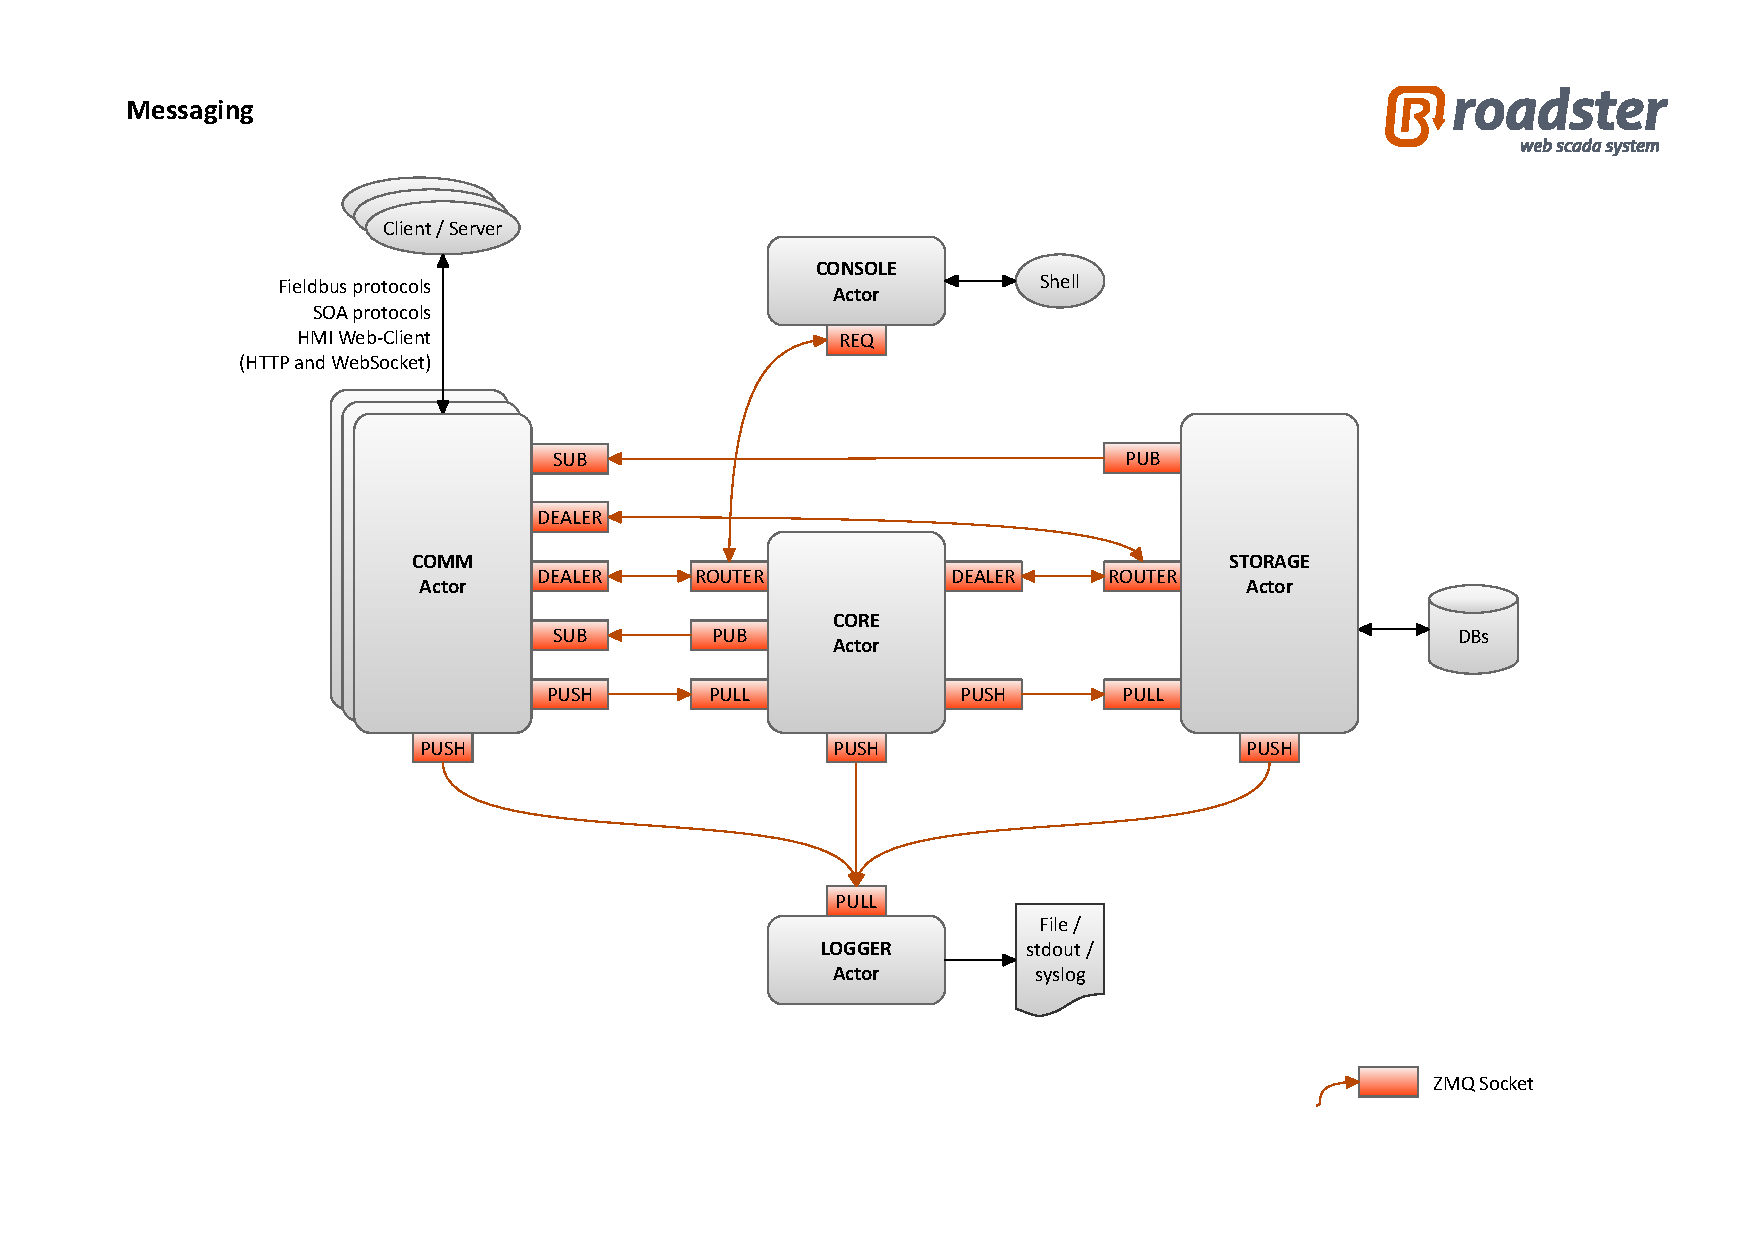
\includegraphics[trim=4cm 2cm 3.5cm 2.8cm, clip=true, width=\textwidth]{img/roadster_arch.pdf}
	\caption{Roadster's software architecture}
	\label{fig:roadster:arch}
\end{figure}

\subsubsection{Communication Layers}
TODO briefly explain layers. \autoref{fig:roadster:layers} illustrates the three layers.

\begin{figure}[!ht]
	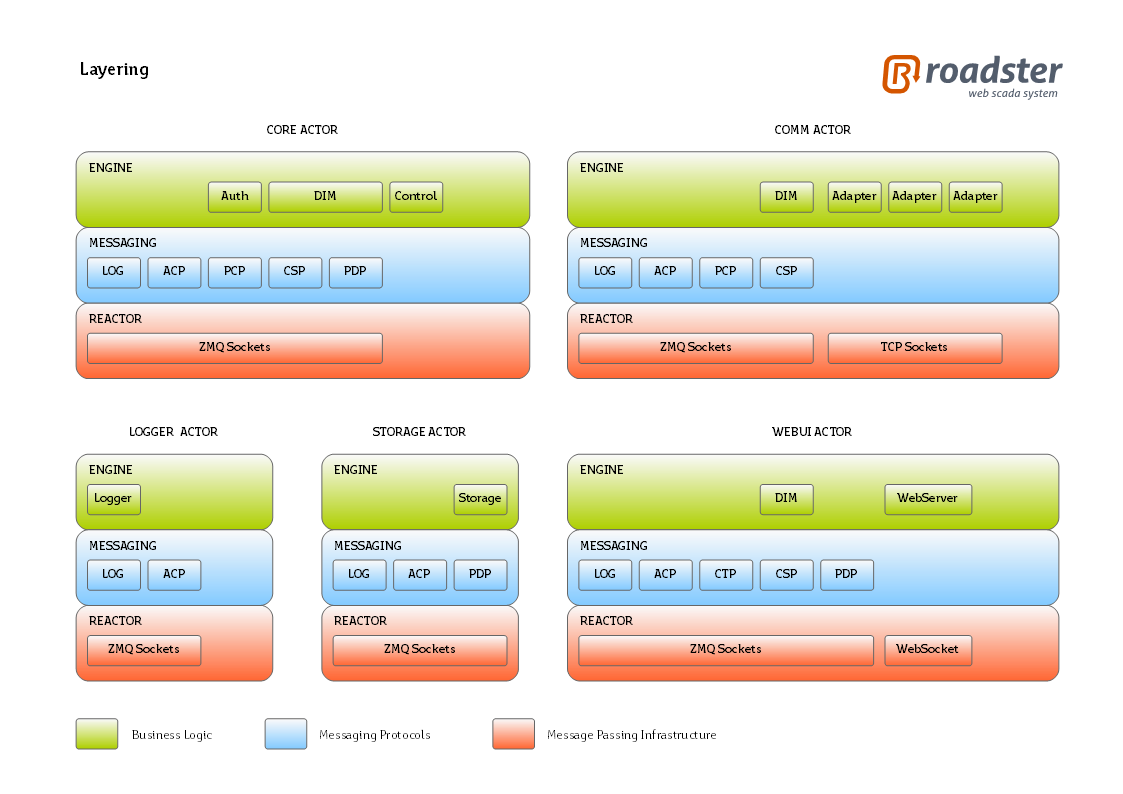
\includegraphics[trim=2cm 2.5cm 1cm 2.8cm, clip=true, width=\textwidth]{img/roadster_layering.png}
	\caption{Roadster's communication layers}
	\label{fig:roadster:layers}
TODO use PDF
\end{figure}

\section{Goals}
TODO mandatory goals

\subsection*{Optional Goals}
TODO optional goals
